\documentclass[a4paper]{article}
\usepackage[margin=0.7in]{geometry}
\usepackage[T1]{fontenc}
\usepackage[utf8]{inputenc}
\usepackage{lmodern}
\usepackage{amsmath}
\usepackage{amssymb}
\usepackage{geometry}
\usepackage{enumerate}
\usepackage{xcolor}
\usepackage{graphicx}
\usepackage{amsthm}
\newtheorem{theorem}{Theorem}[section]
\newtheorem{lemma}[theorem]{Lemma}
\newtheorem{corollary}[theorem]{Corollary}
\newtheorem{definition}[theorem]{Definition}
\usepackage{listings}
\usepackage{authblk}
\usepackage{titling}
\usepackage{zlmtt}
\usepackage{fancyvrb}
\usepackage[hidelinks]{hyperref}
\setlength{\droptitle}{-2em}
\lstset{frame=tb,
  language=C,
  aboveskip=3mm,
  belowskip=3mm,
  showstringspaces=false,   
  columns=flexible,
  basicstyle={\small\ttfamily},
  numbers=none,
  numberstyle=\tiny\color{gray},
  keywordstyle=\color{blue},
  commentstyle=\color{brown},
  stringstyle=\color{orange},
  breaklines=true,
  breakatwhitespace=true,
  tabsize=3
}
\begin{document}
\title{CS3210 Lab 2 Report}
\author{
  Wang Xiyu (A0282500R)
}
\maketitle
\section*{Ex11 Performance Metrics}
This sections shows the comparision of i7-7700(4 cores 8 threads) 
and Xeon Silver 4114 (10 cores 20 cores) in performance measured
 by instruction per cycle(IPC), wall clock time(elapsed time)
  and MFLOPS(Million floating point operations). 
  Both processors have the same core architecture.
\subsection*{Instruction per Cycle}
\par\vspace{3ex}
\begin{minipage}{0.5\linewidth}
    \noindent\makebox[\columnwidth][c]{%
        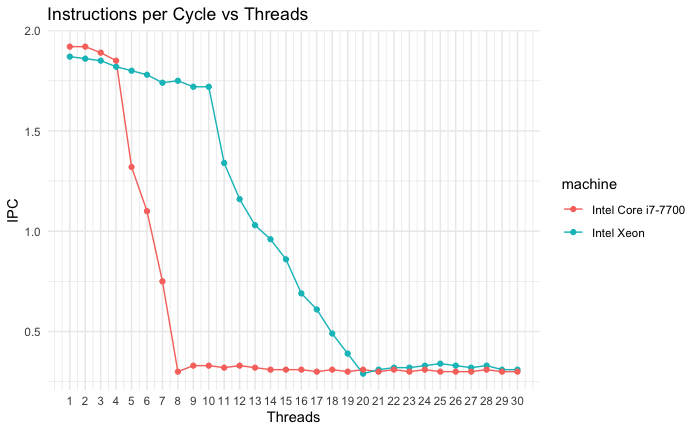
\includegraphics[
        width=\columnwidth,
        clip
        ]{ipc.png}
    }
\end{minipage}\hfill
\begin{minipage}{0.4\linewidth}
    We can observe that for i7-7700 IPC moderately decreases from 1 to 4 threads, and IPC on Xeon 4114 
    also moderately decreases at similar rate from 1 to 10 threads,
    indicating that there exist overhead of thread scheduling 
\end{minipage}\hfill
\subsection*{Wall clock time}
\begin{minipage}{0.5\linewidth}
    \noindent\makebox[\columnwidth][c]{%
  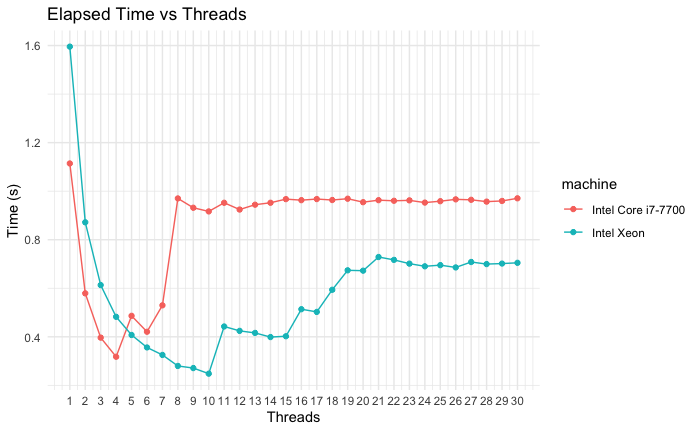
\includegraphics[
    width=\columnwidth,
    trim=0 0 0 0,
    clip
  ]{time.png}
}
\end{minipage}\hfill
\begin{minipage}{0.4\linewidth}
aaa
\end{minipage}\hfill
\par\vspace{3ex}
\subsection*{MFLOPS}
\begin{minipage}{0.5\linewidth}
    \noindent\makebox[\columnwidth][c]{%
    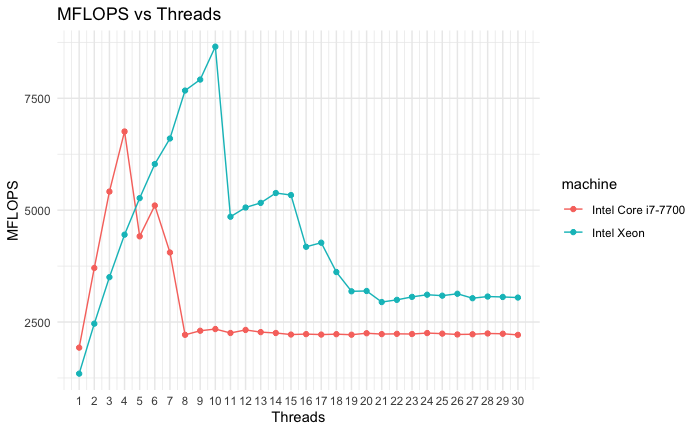
\includegraphics[
      width=\columnwidth,
      trim=0 0 0 0,
      clip
    ]{mflops.png}
    }
\end{minipage}\hfill
\begin{minipage}{0.4\linewidth}
For both processors we can observe that MFLOPS peaks when the number of threads
= the number of cores, this is intuitive as there are more processing units are being utilized and the number of floating 
point operation increases. MFLOPS starts to decrease when number of cores $\leq$ the number of threads $\leq$ 
the number of processing units, this is due to overheads such as memory contention, as both PUs residing in the 
same core share the same LLC (last level cache), causing the overall 
\end{minipage}\hfill



\section*{Ex12\&13 Optimization \& Performance Analysis}
As we can observe from the perf statistics, there are only scalar floating point operations being performed, 
which is a wasted opportunity for SIMD parallelism as we are accessing array elements and we can exploit the spatial locality 
if we can access contiguous cache in consecutive instructions. As 2D arrays are stored row-wise, wwe can access the first matrix by rows, 
but the second matrix is accessed by columns first, ie jumping by \texttt{B.size()}. If we can access matrix B row-wise we can utilize AVX
instructions to perform packed floating point operations. 
\begin{align*}
    AB[i][j] &= \sum_{k=0}^{\texttt{A[0].size()}} A[i][k] \times B[k][j]\\
\end{align*}
We can observe that the order of the accessing order does not matter so long as we ensure in the innermost loop:
\begin{enumerate}
    \item All elements from \texttt{A[i]} and column \texttt{i} of B... 
\end{enumerate}
\par\vspace{3ex}
\begin{minipage}{0.5\linewidth}
\begin{Verbatim}[frame=topline,numbers=left,label= Original,framesep=3mm]
for (i = 0; i < size; i++)
    for (j = 0; j < size; j++)
        for (k = 0; k < size; k++)
            AB[i][j] += A[i][k] * B[k][j];
\end{Verbatim}
\end{minipage}\hfill
\begin{minipage}{0.4\linewidth}
\begin{Verbatim}[frame=topline,numbers=left,label= Optimized,framesep=3mm]
for (i = 0; i < size; i++)
    for (k = 0; k < size; k++)
        for (k = 0; k < size; k++)
            AB[i][j] += A[i][k] * B[k][j];
\end{Verbatim}
\end{minipage}\hfill



\section*{Reproduce result}

compile \& perf sampling options:
\begin{lstlisting}
  g++ mmomp.cpp -o mmomp -fopenmp -O3
  srun perf stat -r 3 -e fp_arith_inst_retired.scalar_single, fp_arith_inst_retired.128b_packed_single, fp_arith_inst_retired.256b_packed_single, cycles,instructions ./mmomp
  g++ rowbase.cpp -o rowbase -fopenmp -O3
  srun perf stat -r 3 -e fp_arith_inst_retired.scalar_single, fp_arith_inst_retired.128b_packed_single, fp_arith_inst_retired.256b_packed_single, cycles, instructions, ./rowbase
\end{lstlisting}

\end{document}